

\documentclass[10pt,xcolor=dvipsnames]{beamer}\usepackage[]{graphicx}\usepackage[]{color}
%% maxwidth is the original width if it is less than linewidth
%% otherwise use linewidth (to make sure the graphics do not exceed the margin)
\makeatletter
\def\maxwidth{ %
  \ifdim\Gin@nat@width>\linewidth
    \linewidth
  \else
    \Gin@nat@width
  \fi
}
\makeatother

\definecolor{fgcolor}{rgb}{0.345, 0.345, 0.345}
\newcommand{\hlnum}[1]{\textcolor[rgb]{0.686,0.059,0.569}{#1}}%
\newcommand{\hlstr}[1]{\textcolor[rgb]{0.192,0.494,0.8}{#1}}%
\newcommand{\hlcom}[1]{\textcolor[rgb]{0.678,0.584,0.686}{\textit{#1}}}%
\newcommand{\hlopt}[1]{\textcolor[rgb]{0,0,0}{#1}}%
\newcommand{\hlstd}[1]{\textcolor[rgb]{0.345,0.345,0.345}{#1}}%
\newcommand{\hlkwa}[1]{\textcolor[rgb]{0.161,0.373,0.58}{\textbf{#1}}}%
\newcommand{\hlkwb}[1]{\textcolor[rgb]{0.69,0.353,0.396}{#1}}%
\newcommand{\hlkwc}[1]{\textcolor[rgb]{0.333,0.667,0.333}{#1}}%
\newcommand{\hlkwd}[1]{\textcolor[rgb]{0.737,0.353,0.396}{\textbf{#1}}}%
\let\hlipl\hlkwb

\usepackage{framed}
\makeatletter
\newenvironment{kframe}{%
 \def\at@end@of@kframe{}%
 \ifinner\ifhmode%
  \def\at@end@of@kframe{\end{minipage}}%
  \begin{minipage}{\columnwidth}%
 \fi\fi%
 \def\FrameCommand##1{\hskip\@totalleftmargin \hskip-\fboxsep
 \colorbox{shadecolor}{##1}\hskip-\fboxsep
     % There is no \\@totalrightmargin, so:
     \hskip-\linewidth \hskip-\@totalleftmargin \hskip\columnwidth}%
 \MakeFramed {\advance\hsize-\width
   \@totalleftmargin\z@ \linewidth\hsize
   \@setminipage}}%
 {\par\unskip\endMakeFramed%
 \at@end@of@kframe}
\makeatother

\definecolor{shadecolor}{rgb}{.97, .97, .97}
\definecolor{messagecolor}{rgb}{0, 0, 0}
\definecolor{warningcolor}{rgb}{1, 0, 1}
\definecolor{errorcolor}{rgb}{1, 0, 0}
\newenvironment{knitrout}{}{} % an empty environment to be redefined in TeX

\usepackage{alltt}
\setbeamertemplate{navigation symbols}{}



\usepackage{color}
\usepackage{CREAL_slides}
\usepackage[latin1]{inputenc}
\usepackage{calc}
\usepackage[loadonly]{enumitem}
\usepackage{float}
\usepackage[position=top,singlelinecheck=off]{subfig}
\usepackage{amsfonts}
\usepackage{amssymb}
\usepackage{amsmath}
\usepackage{tikz}
\usetikzlibrary{arrows}

\DeclareMathOperator{\argmax}{arg\,max}

\newcommand{\X}{\mathbf{X}}



\title[Multivariate methods in health studies]{Supervised Methods  \\ \small{in \\ Methods to integrate multiple tables in biomedical studies to detect biomarkers and stratify individuals \\ \medskip
  Instituto de Salud Carlos III. Centro Nacional de Epidemiolog\'ia \\ September, 2017}}
\author[Juan R Gonzalez]{Juan R Gonzalez}
\institute[CREAL]{BRGE - Bioinformatics Research Group in Epidemiology \\
		  Barcelona Institute for Global Health (ISGlobal) \\
		           {\tt e-mail:juanr.gonzalez@isglobal.org} \\
                  \url{http://www.creal.cat/brge} \\
                  and Departament of Mathematics, UAB
                  }

\date{}
\IfFileExists{upquote.sty}{\usepackage{upquote}}{}
\begin{document}




\frame{\titlepage}


\begin{frame}{Outline}
\tableofcontents
\end{frame}

%%%%%%%%%%%%%%%%%%%%%%%%%%%%%%%%%%%
\section{Supervised methods}
%%%%%%%%%%%%%%%%%%%%%%%%%%%%%%%%%%%


\begin{frame}{Supervised Methods}
\textcolor{blue}{Logistic Regression:} LR Uses a model to predict the probability of having one characteristic or not.
Linear Discriminant Analysis (LDA) can be as an extension of LR (more than two categories in the outcome).
 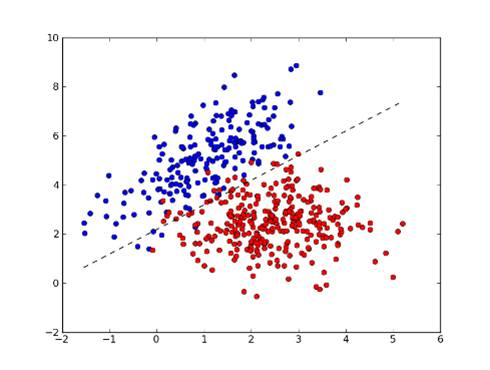
\includegraphics{figures/LR.jpg}
\end{frame}

\begin{frame}{Supervised Methods}
\textcolor{blue}{Classification Trees:}  A tree model resembles that of a linear model, 
where the criterion is the factor indicating class membership and the predictor variables are the
observed values for each variable.

\medskip
 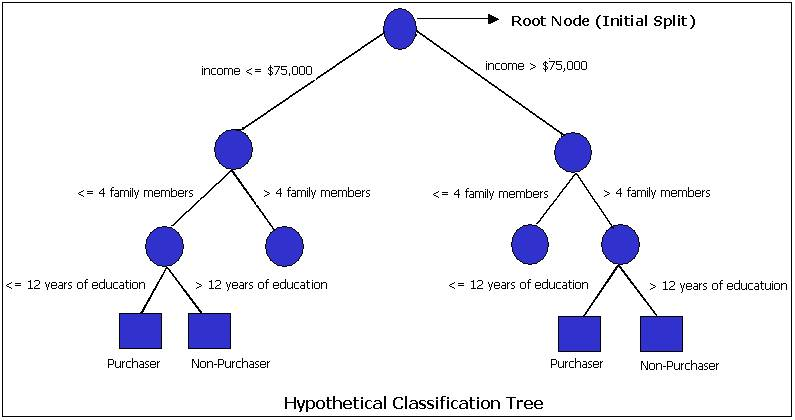
\includegraphics{figures/tree.jpg}
\end{frame}


\begin{frame}{Supervised Methods}
\textcolor{blue}{Support Vector Machine:} SVM finds separating lines (hyper planes) between groups of points.
\bigskip
 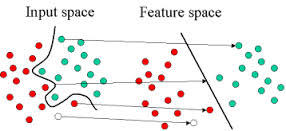
\includegraphics{figures/svm.jpg}
\end{frame}


\begin{frame}{Supervised Methods}
\textcolor{blue}{Neural Networks:} Nonlinear models consisting of  hyperplanes around  classes of objects given a set of prediction variables finds separating lines (hyper planes) between groups of points.
 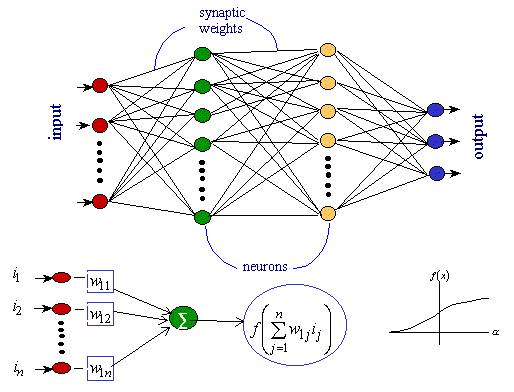
\includegraphics{figures/NN.jpg}
\end{frame}


\begin{frame}{Supervised Methods}
\textcolor{blue}{Boosting:} Boosting is a combination of weak classifiers to produce a 
   powerful committee. 

\bigskip
 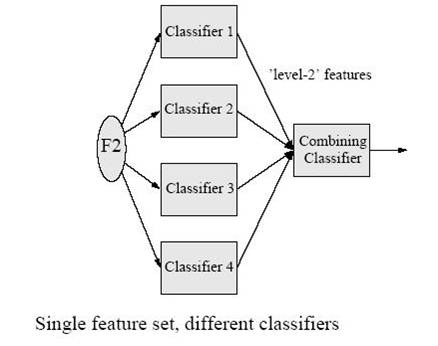
\includegraphics{figures/boosting.jpg}
\end{frame}

\begin{frame}{Supervised Methods}
\textcolor{blue}{Random Forest:} It can be seen as an extension of Boosting when using trees as a classifiers.

\bigskip
 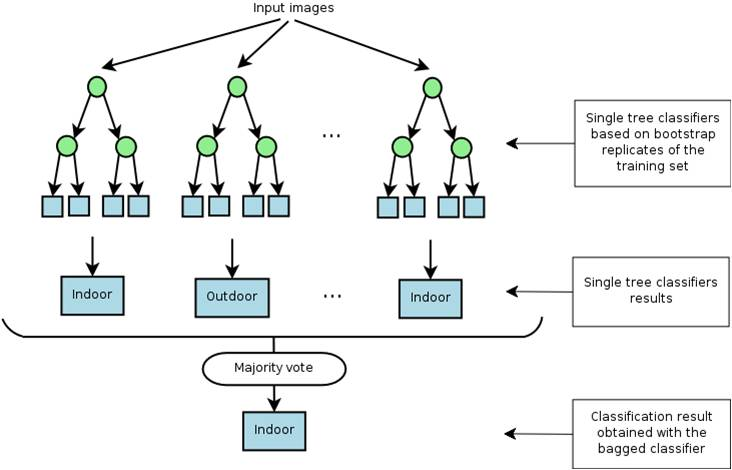
\includegraphics{figures/RF.jpg}
\end{frame}


\begin{frame}[fragile]{Supervised methods}
\textbf{Example:} {\tt oliveoil} data set represents eight chemical measurements 
on different specimen of olive oil produced in various regions in 
Italy (northern Apulia, southern Apulia, Calabria, Sicily, inland Sardinia 
and coast Sardinia, eastern and western Liguria, Umbria) and further 
classifiable into three macro-areas: Centre-North, South, Sardinia. 

\begin{knitrout}\footnotesize
\definecolor{shadecolor}{rgb}{0.969, 0.969, 0.969}\color{fgcolor}\begin{kframe}
\begin{alltt}
\hlkwd{library}\hlstd{(pdfCluster)}
\hlkwd{data}\hlstd{(oliveoil)}
\hlkwd{head}\hlstd{(oliveoil)}
\end{alltt}
\begin{verbatim}
##   macro.area       region palmitic palmitoleic stearic oleic linoleic linolenic
## 1      South Apulia.north     1075          75     226  7823      672        36
## 2      South Apulia.north     1088          73     224  7709      781        31
## 3      South Apulia.north      911          54     246  8113      549        31
## 4      South Apulia.north      966          57     240  7952      619        50
## 5      South Apulia.north     1051          67     259  7771      672        50
## 6      South Apulia.north      911          49     268  7924      678        51
##   arachidic eicosenoic
## 1        60         29
## 2        61         29
## 3        63         29
## 4        78         35
## 5        80         46
## 6        70         44
\end{verbatim}
\end{kframe}
\end{knitrout}
\end{frame}


\begin{frame}[fragile]{Supervised methods}
\begin{knitrout}\footnotesize
\definecolor{shadecolor}{rgb}{0.969, 0.969, 0.969}\color{fgcolor}\begin{kframe}
\begin{alltt}
\hlkwd{set.seed}\hlstd{(}\hlnum{1234}\hlstd{)}
\hlstd{ss} \hlkwb{<-} \hlkwd{sample}\hlstd{(}\hlnum{1}\hlopt{:}\hlkwd{nrow}\hlstd{(oliveoil),} \hlnum{200}\hlstd{)}
\hlstd{train} \hlkwb{<-} \hlstd{oliveoil[}\hlopt{-}\hlstd{ss,}\hlopt{-}\hlnum{2}\hlstd{]}
\hlstd{test} \hlkwb{<-} \hlstd{oliveoil[ss,}\hlopt{-}\hlnum{2}\hlstd{]}
\end{alltt}
\end{kframe}
\end{knitrout}
\end{frame}



\begin{frame}[fragile]{Linear discriminant analysis}
\begin{knitrout}\footnotesize
\definecolor{shadecolor}{rgb}{0.969, 0.969, 0.969}\color{fgcolor}\begin{kframe}
\begin{alltt}
\hlkwd{library}\hlstd{(MASS)}
\hlstd{olive.lda} \hlkwb{<-} \hlkwd{lda}\hlstd{(macro.area}\hlopt{~}\hlstd{., train)}
\hlstd{pregion.lda} \hlkwb{<-} \hlkwd{predict}\hlstd{(olive.lda, test)}\hlopt{$}\hlstd{class}
\hlkwd{table}\hlstd{(test[,}\hlnum{1}\hlstd{], pregion.lda)}
\end{alltt}
\begin{verbatim}
##               pregion.lda
##                South Sardinia Centre.North
##   South          116        0            0
##   Sardinia         0       35            0
##   Centre.North     0        1           48
\end{verbatim}
\end{kframe}
\end{knitrout}
\end{frame}



\begin{frame}[fragile]{Linear discriminant analysis}
\begin{knitrout}\footnotesize
\definecolor{shadecolor}{rgb}{0.969, 0.969, 0.969}\color{fgcolor}\begin{kframe}
\begin{alltt}
\hlkwd{plot}\hlstd{(}\hlkwd{predict}\hlstd{(olive.lda, test)}\hlopt{$}\hlstd{x,}
     \hlkwc{col}\hlstd{=}\hlkwd{as.numeric}\hlstd{(test[,}\hlnum{1}\hlstd{]))}
\end{alltt}
\end{kframe}

{\centering 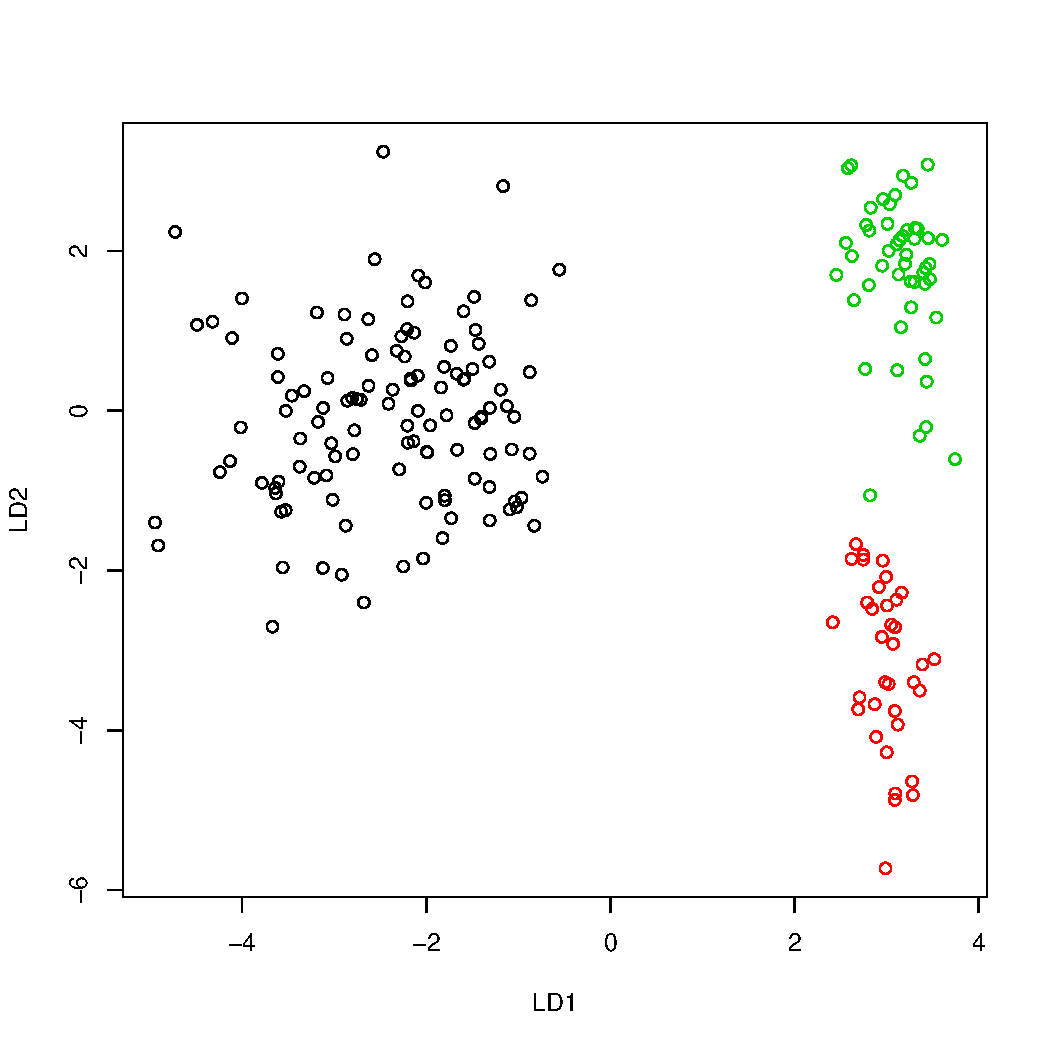
\includegraphics[width=2in]{figure/ldaPlot-1} 

}



\end{knitrout}
\end{frame}


\begin{frame}[fragile]{Classification Trees}
\begin{knitrout}\footnotesize
\definecolor{shadecolor}{rgb}{0.969, 0.969, 0.969}\color{fgcolor}\begin{kframe}
\begin{alltt}
\hlkwd{library}\hlstd{(rpart)}
\hlstd{olive.rp} \hlkwb{<-} \hlkwd{rpart}\hlstd{(macro.area}\hlopt{~}\hlstd{., train,}
          \hlkwc{method}\hlstd{=}\hlstr{"class"}\hlstd{)}
\hlstd{olive.rp}
\end{alltt}
\begin{verbatim}
## n= 372 
## 
## node), split, n, loss, yval, (yprob)
##       * denotes terminal node
## 
## 1) root 372 165 South (0.5564516 0.1693548 0.2741935)  
##   2) eicosenoic>=6.5 207   0 South (1.0000000 0.0000000 0.0000000) *
##   3) eicosenoic< 6.5 165  63 Centre.North (0.0000000 0.3818182 0.6181818)  
##     6) oleic< 7438.5 63   0 Sardinia (0.0000000 1.0000000 0.0000000) *
##     7) oleic>=7438.5 102   0 Centre.North (0.0000000 0.0000000 1.0000000) *
\end{verbatim}
\end{kframe}
\end{knitrout}
\end{frame}


\begin{frame}[fragile]{Classification Trees}
\begin{knitrout}\footnotesize
\definecolor{shadecolor}{rgb}{0.969, 0.969, 0.969}\color{fgcolor}\begin{kframe}
\begin{alltt}
\hlkwd{plot}\hlstd{(olive.rp)}
\hlkwd{text}\hlstd{(olive.rp)}
\end{alltt}
\end{kframe}

{\centering 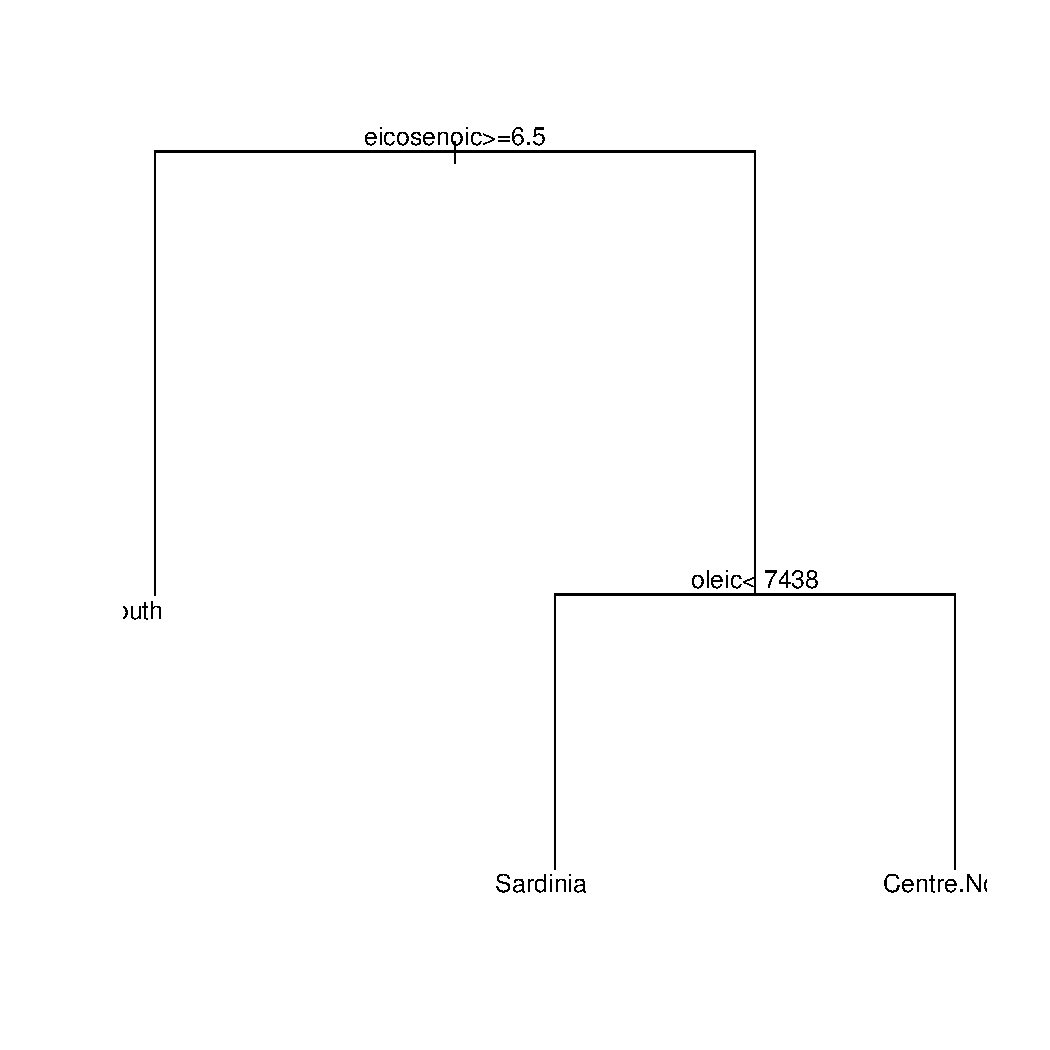
\includegraphics[width=2in]{figure/treesPlot-1} 

}



\end{knitrout}
\end{frame}

\begin{frame}[fragile]{Linear discriminant analysis}
\begin{knitrout}\footnotesize
\definecolor{shadecolor}{rgb}{0.969, 0.969, 0.969}\color{fgcolor}\begin{kframe}
\begin{alltt}
\hlstd{temp} \hlkwb{<-} \hlkwd{predict}\hlstd{(olive.rp, test)}
\hlkwd{head}\hlstd{(temp)}
\end{alltt}
\begin{verbatim}
##     South Sardinia Centre.North
## 66      1        0            0
## 356     0        1            0
## 348     0        1            0
## 355     0        1            0
## 489     0        0            1
## 364     0        1            0
\end{verbatim}
\begin{alltt}
\hlstd{pregion.rp} \hlkwb{<-} \hlkwd{apply}\hlstd{(temp,} \hlnum{1}\hlstd{,} \hlkwa{function}\hlstd{(}\hlkwc{x}\hlstd{)} \hlkwd{which}\hlstd{(x}\hlopt{==}\hlnum{1}\hlstd{))}
\end{alltt}
\end{kframe}
\end{knitrout}
\end{frame}

\begin{frame}[fragile]{Linear discriminant analysis}
\begin{knitrout}\footnotesize
\definecolor{shadecolor}{rgb}{0.969, 0.969, 0.969}\color{fgcolor}\begin{kframe}
\begin{alltt}
\hlkwd{table}\hlstd{(test[,}\hlnum{1}\hlstd{], pregion.rp)}
\end{alltt}
\begin{verbatim}
##               pregion.rp
##                  1   2   3
##   South        116   0   0
##   Sardinia       0  34   1
##   Centre.North   0   2  47
\end{verbatim}
\end{kframe}
\end{knitrout}
\end{frame}

\begin{frame}[fragile]{Support Vector Machine}
\begin{knitrout}\footnotesize
\definecolor{shadecolor}{rgb}{0.969, 0.969, 0.969}\color{fgcolor}\begin{kframe}
\begin{alltt}
\hlkwd{library}\hlstd{(e1071)}
\hlstd{olive.svm} \hlkwb{<-}  \hlkwd{svm}\hlstd{(macro.area} \hlopt{~}\hlstd{. ,} \hlkwc{data} \hlstd{= train)}
\hlstd{pregion.svm} \hlkwb{<-} \hlkwd{predict}\hlstd{(olive.svm, test)}
\hlkwd{table}\hlstd{(test[,}\hlnum{1}\hlstd{], pregion.svm)}
\end{alltt}
\begin{verbatim}
##               pregion.svm
##                South Sardinia Centre.North
##   South          116        0            0
##   Sardinia         0       35            0
##   Centre.North     0        0           49
\end{verbatim}
\end{kframe}
\end{knitrout}
\end{frame}

\begin{frame}[fragile]{Neural Network}
\begin{knitrout}\footnotesize
\definecolor{shadecolor}{rgb}{0.969, 0.969, 0.969}\color{fgcolor}\begin{kframe}
\begin{alltt}
\hlkwd{library}\hlstd{(nnet)}
\hlstd{olive.nnet} \hlkwb{<-}  \hlkwd{nnet}\hlstd{(macro.area} \hlopt{~}\hlstd{. ,} \hlkwc{data} \hlstd{= train,}
               \hlkwc{size}\hlstd{=}\hlnum{2}\hlstd{)}
\end{alltt}
\begin{verbatim}
## # weights:  27
## initial  value 463.503444 
## final  value 365.191009 
## converged
\end{verbatim}
\begin{alltt}
\hlstd{pregion.nnet} \hlkwb{<-} \hlkwd{predict}\hlstd{(olive.nnet, test,} \hlkwc{type}\hlstd{=}\hlstr{"class"}\hlstd{)}
\hlkwd{table}\hlstd{(test[,}\hlnum{1}\hlstd{], pregion.nnet)}
\end{alltt}
\begin{verbatim}
##               pregion.nnet
##                South
##   South          116
##   Sardinia        35
##   Centre.North    49
\end{verbatim}
\end{kframe}
\end{knitrout}
\end{frame}

\begin{frame}[fragile]{Neural Network}
\begin{knitrout}\footnotesize
\definecolor{shadecolor}{rgb}{0.969, 0.969, 0.969}\color{fgcolor}\begin{kframe}
\begin{alltt}
\hlstd{olive.nnet} \hlkwb{<-}  \hlkwd{nnet}\hlstd{(macro.area} \hlopt{~}\hlstd{. ,} \hlkwc{data} \hlstd{= train,}
               \hlkwc{size}\hlstd{=}\hlnum{4}\hlstd{)}
\end{alltt}
\begin{verbatim}
## # weights:  51
## initial  value 539.582101 
## final  value 365.191009 
## converged
\end{verbatim}
\begin{alltt}
\hlstd{pregion.nnet} \hlkwb{<-} \hlkwd{predict}\hlstd{(olive.nnet, test,} \hlkwc{type}\hlstd{=}\hlstr{"class"}\hlstd{)}
\hlkwd{table}\hlstd{(test[,}\hlnum{1}\hlstd{], pregion.nnet)}
\end{alltt}
\begin{verbatim}
##               pregion.nnet
##                South
##   South          116
##   Sardinia        35
##   Centre.North    49
\end{verbatim}
\end{kframe}
\end{knitrout}
\end{frame}


\begin{frame}[fragile]{Boosting}
\begin{knitrout}\footnotesize
\definecolor{shadecolor}{rgb}{0.969, 0.969, 0.969}\color{fgcolor}\begin{kframe}
\begin{alltt}
\hlkwd{library}\hlstd{(adabag)}
\hlstd{olive.boost} \hlkwb{<-}  \hlkwd{boosting}\hlstd{(macro.area} \hlopt{~}\hlstd{. ,} \hlkwc{data} \hlstd{= train,}
                \hlkwc{control} \hlstd{=} \hlkwd{rpart.control}\hlstd{(}\hlkwc{maxdepth} \hlstd{=} \hlnum{2}\hlstd{))}
\hlstd{pregion.boost} \hlkwb{<-} \hlkwd{predict}\hlstd{(olive.boost, test,} \hlkwc{type}\hlstd{=}\hlstr{"class"}\hlstd{)}\hlopt{$}\hlstd{class}
\hlkwd{table}\hlstd{(test[,}\hlnum{1}\hlstd{], pregion.boost)}
\end{alltt}
\begin{verbatim}
##               pregion.boost
##                Centre.North Sardinia South
##   South                   0        0   116
##   Sardinia                1       34     0
##   Centre.North           47        2     0
\end{verbatim}
\end{kframe}
\end{knitrout}
\end{frame}

\begin{frame}[fragile]{Random Forest}
\begin{knitrout}\footnotesize
\definecolor{shadecolor}{rgb}{0.969, 0.969, 0.969}\color{fgcolor}\begin{kframe}
\begin{alltt}
\hlkwd{library}\hlstd{(randomForest)}
\hlstd{olive.rf} \hlkwb{<-}  \hlkwd{randomForest}\hlstd{(macro.area} \hlopt{~}\hlstd{. ,} \hlkwc{data} \hlstd{= train)}
\hlstd{pregion.rf} \hlkwb{<-} \hlkwd{predict}\hlstd{(olive.rf, test,} \hlkwc{type}\hlstd{=}\hlstr{"class"}\hlstd{)}
\hlkwd{table}\hlstd{(test[,}\hlnum{1}\hlstd{], pregion.rf)}
\end{alltt}
\begin{verbatim}
##               pregion.rf
##                South Sardinia Centre.North
##   South          116        0            0
##   Sardinia         0       35            0
##   Centre.North     0        0           49
\end{verbatim}
\end{kframe}
\end{knitrout}
\end{frame}



%%%%%%%%%%%%%%%%%%%%%%%%%%%%%%%%%%%
\section{Model performance}
%%%%%%%%%%%%%%%%%%%%%%%%%%%%%%%%%%%

\begin{frame}[fragile]{Model performance}
 \begin{itemize}
   \item Rand Index (categorical biomarker)
   \item ROC curve (continuous biomarker)
 \end{itemize}
\end{frame}




\begin{frame}[fragile]{Model performance}
\textbf{Rand Index: used in the class prediction problem}
\begin{knitrout}\footnotesize
\definecolor{shadecolor}{rgb}{0.969, 0.969, 0.969}\color{fgcolor}\begin{kframe}
\begin{alltt}
\hlkwd{library}\hlstd{(flexclust)}
\hlkwd{randIndex}\hlstd{(}\hlkwd{table}\hlstd{(test[,}\hlnum{1}\hlstd{], pregion.rf))}
\end{alltt}
\begin{verbatim}
## ARI 
##   1
\end{verbatim}
\begin{alltt}
\hlkwd{randIndex}\hlstd{(}\hlkwd{table}\hlstd{(test[,}\hlnum{1}\hlstd{], pregion.lda))}
\end{alltt}
\begin{verbatim}
##       ARI 
## 0.9914602
\end{verbatim}
\begin{alltt}
\hlkwd{randIndex}\hlstd{(}\hlkwd{table}\hlstd{(test[,}\hlnum{1}\hlstd{], pregion.rp))}
\end{alltt}
\begin{verbatim}
##       ARI 
## 0.9749979
\end{verbatim}
\begin{alltt}
\hlkwd{randIndex}\hlstd{(}\hlkwd{table}\hlstd{(test[,}\hlnum{1}\hlstd{], pregion.boost))}
\end{alltt}
\begin{verbatim}
##       ARI 
## 0.9749979
\end{verbatim}
\end{kframe}
\end{knitrout}
\end{frame}





\begin{frame}[fragile]{Model performance}
Let us assume that we want to use different biomarkers (continuous) to predict and outcome. For instance, researchers want to use several clinical and one laboratory variable to predict 6-month outcome (Good and Poor) after having an aneurysmal subarachnoid haemorrhage (aSAH). These are the variables the collected at hospital admission

\begin{knitrout}\footnotesize
\definecolor{shadecolor}{rgb}{0.969, 0.969, 0.969}\color{fgcolor}\begin{kframe}
\begin{alltt}
\hlkwd{library}\hlstd{(pROC)}
\hlkwd{data}\hlstd{(aSAH)}
\hlkwd{head}\hlstd{(aSAH)}
\end{alltt}
\begin{verbatim}
##    gos6 outcome gender age wfns s100b  ndka
## 29    5    Good Female  42    1  0.13  3.01
## 30    5    Good Female  37    1  0.14  8.54
## 31    5    Good Female  42    1  0.10  8.09
## 32    5    Good Female  27    1  0.04 10.42
## 33    1    Poor Female  42    3  0.13 17.40
## 34    1    Poor   Male  48    2  0.10 12.75
\end{verbatim}
\end{kframe}
\end{knitrout}

\end{frame}



\begin{frame}[fragile]{Model performance}
Let us assume that we want to compute the AUC and its confidence interval for a given biomarker

\begin{knitrout}\footnotesize
\definecolor{shadecolor}{rgb}{0.969, 0.969, 0.969}\color{fgcolor}\begin{kframe}
\begin{alltt}
\hlstd{rocobj} \hlkwb{<-} \hlkwd{plot.roc}\hlstd{(aSAH}\hlopt{$}\hlstd{outcome, aSAH}\hlopt{$}\hlstd{s100b,}
                \hlkwc{main}\hlstd{=}\hlstr{"Confidence intervals"}\hlstd{,}
                \hlkwc{percent}\hlstd{=}\hlnum{TRUE}\hlstd{,}
                \hlkwc{ci}\hlstd{=}\hlnum{TRUE}\hlstd{,}
                \hlkwc{print.auc}\hlstd{=}\hlnum{TRUE}\hlstd{)}
\end{alltt}
\end{kframe}

{\centering 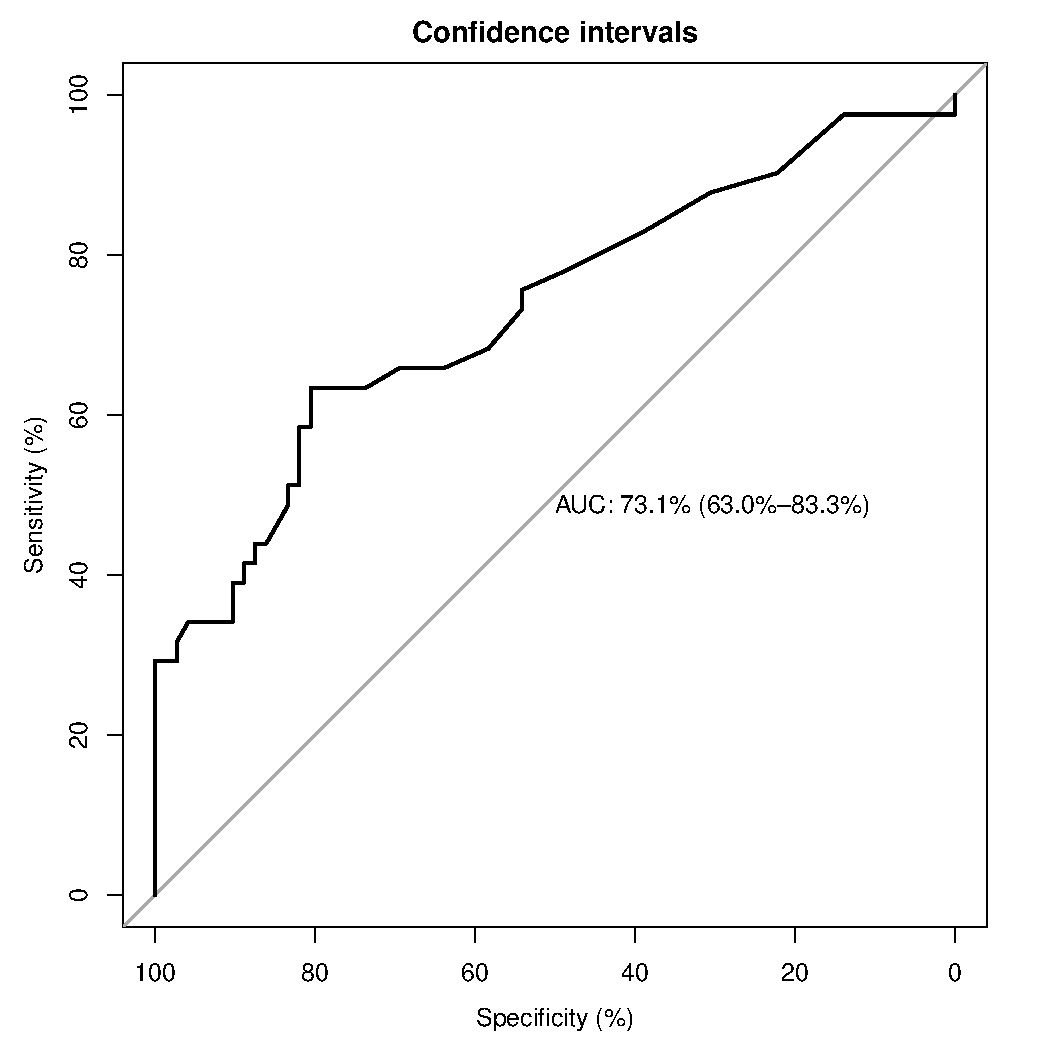
\includegraphics[width=2in]{figure/ROC_2-1} 

}



\end{knitrout}

\end{frame}



\begin{frame}[fragile]{Model performance}
A confidence band can be added

\begin{knitrout}\footnotesize
\definecolor{shadecolor}{rgb}{0.969, 0.969, 0.969}\color{fgcolor}\begin{kframe}
\begin{alltt}
\hlstd{rocobj} \hlkwb{<-} \hlkwd{plot.roc}\hlstd{(aSAH}\hlopt{$}\hlstd{outcome, aSAH}\hlopt{$}\hlstd{s100b,}
                \hlkwc{main}\hlstd{=}\hlstr{"Confidence intervals"}\hlstd{,} \hlkwc{percent}\hlstd{=}\hlnum{TRUE}\hlstd{,}
                \hlkwc{ci}\hlstd{=}\hlnum{TRUE}\hlstd{,}
                \hlkwc{print.auc}\hlstd{=}\hlnum{TRUE}\hlstd{)}
\hlstd{ciobj} \hlkwb{<-} \hlkwd{ci.se}\hlstd{(rocobj,} \hlkwc{progress} \hlstd{=} \hlstr{"none"}\hlstd{,}
               \hlkwc{specificities}\hlstd{=}\hlkwd{seq}\hlstd{(}\hlnum{0}\hlstd{,} \hlnum{100}\hlstd{,} \hlnum{5}\hlstd{))} \hlcom{#This can be selected (grid for computing bands)}
\hlkwd{plot}\hlstd{(ciobj,} \hlkwc{type}\hlstd{=}\hlstr{"shape"}\hlstd{,} \hlkwc{col}\hlstd{=}\hlstr{"lightblue"}\hlstd{)} \hlcom{# plot as a blue shape}
\end{alltt}
\end{kframe}

{\centering 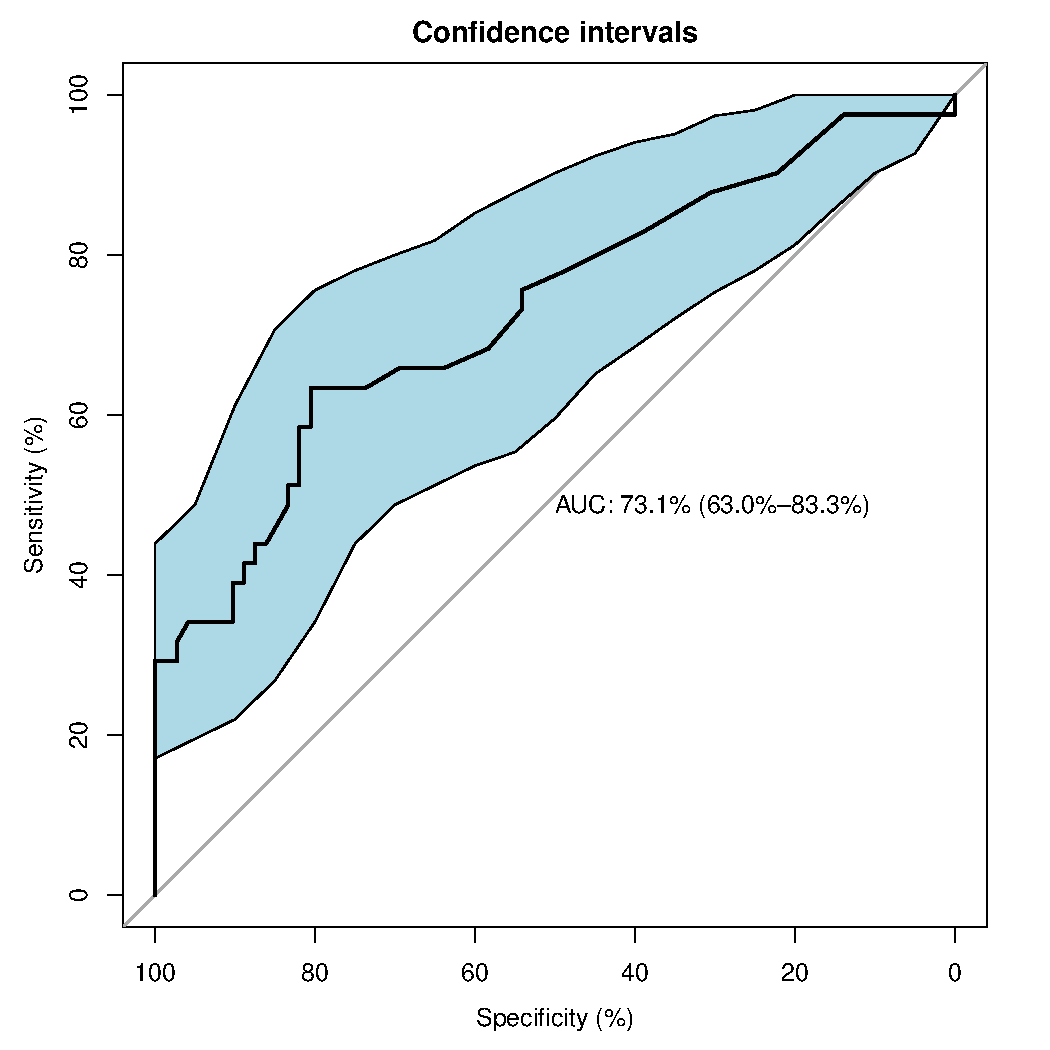
\includegraphics[width=2in]{figure/ROC_3-1} 

}



\end{knitrout}

\end{frame}



\begin{frame}[fragile]{Model performance}

Two biomarkers can be compared by

\begin{knitrout}\footnotesize
\definecolor{shadecolor}{rgb}{0.969, 0.969, 0.969}\color{fgcolor}\begin{kframe}
\begin{alltt}
\hlstd{rocobj1} \hlkwb{<-} \hlkwd{plot.roc}\hlstd{(aSAH}\hlopt{$}\hlstd{outcome, aSAH}\hlopt{$}\hlstd{s100,}
                    \hlkwc{main}\hlstd{=}\hlstr{"Statistical comparison"}\hlstd{,} \hlkwc{percent}\hlstd{=}\hlnum{TRUE}\hlstd{,} \hlkwc{col}\hlstd{=}\hlstr{"blue"}\hlstd{)}
\hlstd{rocobj2} \hlkwb{<-} \hlkwd{lines.roc}\hlstd{(aSAH}\hlopt{$}\hlstd{outcome, aSAH}\hlopt{$}\hlstd{ndka,} \hlkwc{percent}\hlstd{=}\hlnum{TRUE}\hlstd{,} \hlkwc{col}\hlstd{=}\hlstr{"red"}\hlstd{)}
\hlstd{testobj} \hlkwb{<-} \hlkwd{roc.test}\hlstd{(rocobj1, rocobj2)}
\hlkwd{text}\hlstd{(}\hlnum{50}\hlstd{,} \hlnum{50}\hlstd{,} \hlkwc{labels}\hlstd{=}\hlkwd{paste}\hlstd{(}\hlstr{"p-value ="}\hlstd{,} \hlkwd{format.pval}\hlstd{(testobj}\hlopt{$}\hlstd{p.value)),} \hlkwc{adj}\hlstd{=}\hlkwd{c}\hlstd{(}\hlnum{0}\hlstd{,} \hlnum{.5}\hlstd{))}
\hlkwd{legend}\hlstd{(}\hlstr{"bottomright"}\hlstd{,} \hlkwc{legend}\hlstd{=}\hlkwd{c}\hlstd{(}\hlstr{"S100B"}\hlstd{,} \hlstr{"NDKA"}\hlstd{),} \hlkwc{col}\hlstd{=}\hlkwd{c}\hlstd{(}\hlstr{"blue"}\hlstd{,} \hlstr{"red"}\hlstd{),} \hlkwc{lwd}\hlstd{=}\hlnum{2}\hlstd{)}
\end{alltt}
\end{kframe}

{\centering 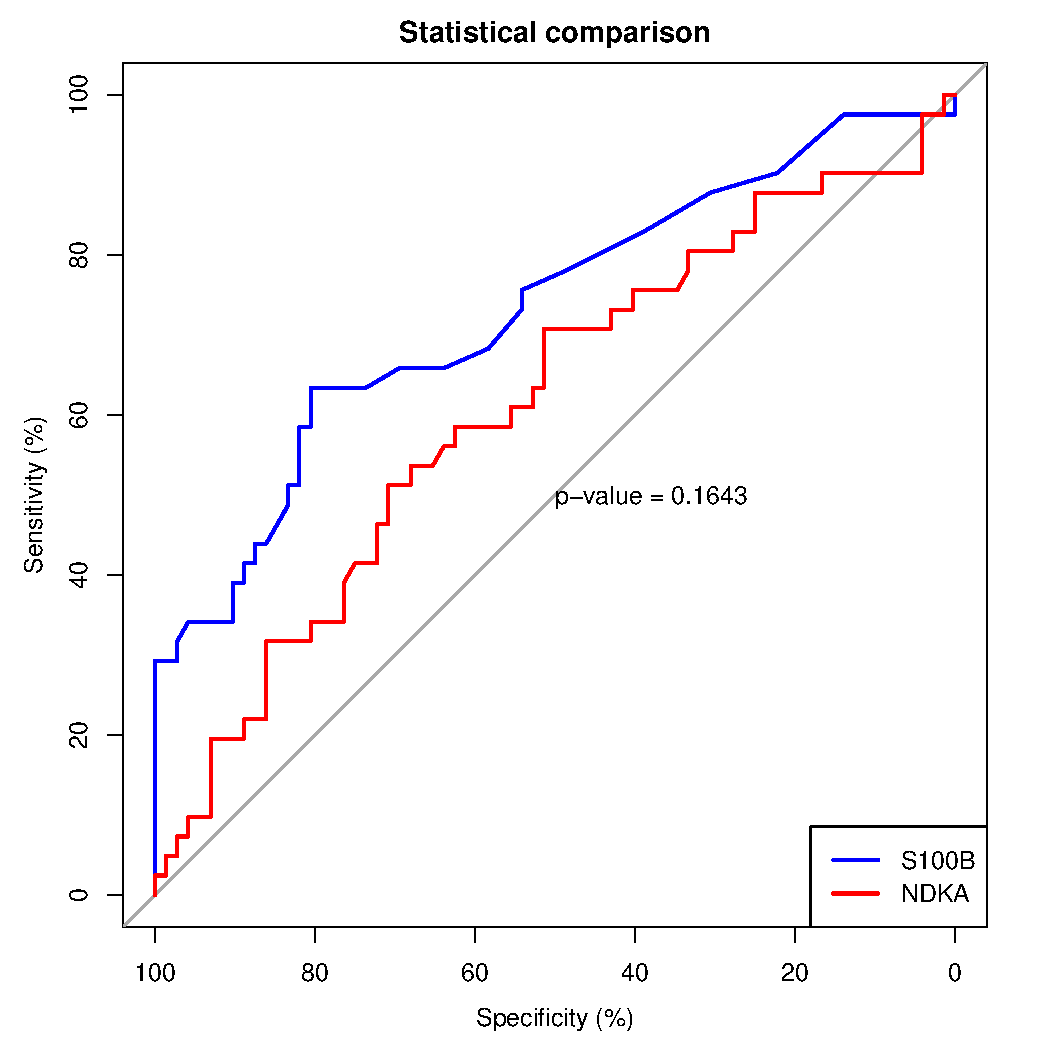
\includegraphics[width=2in]{figure/compareAUC-1} 

}



\end{knitrout}
\end{frame}






\end{document}





